\chapter{Introduction}
\label{chapter-introduction}

A \newterm{wireless sensor network} (WSN) is a network composed of small sensors or actuators
that are connected by way of short hop wireless links. Commonly such networks include one or
more base stations with wider connectivity that serve as an interface between the sensor network
and external systems. WSNs are an area of intense study with many envisioned applications
ranging from environment, asset, and structural monitoring to emergency response
\cite{Culler:2004:GEI:1018015.1018072,1038146}.

Sensor networks, like any small embedded system, present difficult programming challenges
\cite{Mottola:2011:PWS:1922649.1922656}. For reasons of size, power consumption, disposability,
or some combination of these things, sensor network nodes are often highly resource constrained.
A typical node might have only 48~KiB of program ROM, 8~KiB of RAM (or less), and be using a
small, 16~bit microcontroller running at only 8~MHz \cite{tmotesky-datasheet}. Yet WSN
applications are increasing in complexity. In addition to application logic, such systems are
now expected to support facilities such as IPv6 \cite{Hui:2008:IDL:1460412.1460415} and
elaborate security services \cite{perrig-2004}, as just two examples.

My interest is in discovering how to effectively program these limited devices to meet high
level security goals. While there has been a great deal of research on security in sensor
networks much of that work has focused on low level concerns such as link layer security, key
distribution \cite{camtepe-bulent-05}, and secure network protocols
\cite{1049776,fouladgar-3tls-2006}. Systems such as TinySec \cite{karlog-tinysec-2004} and
MiniSec \cite{luk-minisec-2007} are based on shared secrets and generally assume that an entire
network comprises a single security domain. Furthermore, these systems support confidentiality
and integrity properties, but not access control, aka authorization.

The purpose of my work is, rather, to support high level authorization policies that allow a
network in one security domain to grant selective access to its resources by nodes in a
cooperating security domain. Such distributed authorization systems, called \newterm{trust
  management systems} have also been an active area of research
\cite{chapin-skalka-wang-acmcs08}.

A trust management system typically entails the use of public key cryptography to allow
principals to authorize each other without prior introduction and a system for evaluating
authorization requests in the light of some access policy. Although the feasibility of using
public key cryptography on sensor nodes has been shown by several authors
\cite{1049776,Malan:2008:IPI:1387663.1387668,bertoni-2006,kumar-2006,4604657,Liu-Peng-TinyECC-2008,Szczechowiak:2008:NTL:1786014.1786040},
combining this with the necessary authorization computations to support a full trust management
system, and showing the feasibility and practicality of doing so, has not been previously
demonstrated.

Here I describe two approaches to solving the problem of providing trust management-style
distributed authorization in WSNs. The first approach is based on a new RPC discipline called
\textit{SpartanRPC}. In this method all cryptographic and authorization computations are done on
the sensor nodes directly. However, the complexity of the system is hidden from the programmer
behind an easy to use extension of the widely used nesC programming language
\cite{Gay-nesC-2003}. My implementation of this direct approach is a compiler called
\textit{Sprocket} that takes an extended dialect of the nesC language as input and outputs an
equivalent program in regular nesC. In addition Sprocket outputs the necessary runtime support
to process authorization requests and policy statements in the previously developed $RT_0$ trust
management language \cite{Li:DRBTMF,Li:RRBTMF}.

The second approach I present is based on \newterm{staged programming}. In a staged environment,
a first stage program is used to compose and specialize a lower level, second stage program.
Specialized code can often be considerably optimized. However, flexibility is retained because
the first stage program can be re-executed at a later time to re-specialize the second stage
code as needed.

Staging is a widely researched topic
\cite{Taha-MetaML,Sheard-TemplateHaskell,Mainland-Flask-2008,FramedML}. Many staged programming
systems are quite general and allow an arbitrary number of stages where each stage can
manipulate small fragments of next-stage code. Furthermore the type correctness of the stage
$n+1$ programs are normally checked during their compilation or during the execution of the
stage $n$ programs that produce them.

I focus here on the specific problem of using staged programming to improve the efficiency of
node level programs for wireless sensor networks. In such an environment I envision the first
stage program as running on a powerful base station (also called a ``hub'') or even a hand-held
device such as a smart phone. Potentially using information gathered in the field, the first
stage program computes an appropriately specialized second stage program that is then deployed
to the network using an in-situ distributed deployment system such as Deluge \cite{deluge04}.
Feedback provided by the network allows the first stage program to recompute an updated second
stage program that can then be redeployed over the air.

In this environment only two stages are necessary so a language that provides an arbitrary
number of stages is not required. Furthermore the practical realities of sensor network
programming means that the second stage language needs to be either C or nesC or some dialect of
these languages. However, nesC, especially, is an embedded systems language and not suitable for
creating high level applications. Thus the first stage language can and should be something
more appropriate to its task.

In this dissertation I describe \newterm{Scalaness}, an extension of Scala \cite{PiS2} with
features that allow the programmer to compose and specialize components written in a reduced
dialect of nesC called \newterm{nesT}. One novel feature of Scalaness is that the type system of
Scala has been extended so that a well-typed Scalaness program will always generate a well-typed
nesT program \cite{chapin-GPCE-2013}.

\autoref{figure-scalaness} provides an overview of the Scalaness/nesT language
architecture. Scalaness source code is compiled in a modified Scala compiler to Java bytecode,
and run in a standard JVM. At runtime this Scalaness program may generate nesT code, which is
subsequently rewritten to nesC and compiled using the standard TinyOS compiler. The resulting
image can then be installed on sensor network nodes.

\begin{fpfig*}[t]
  {Scalaness/nesT Compilation and Execution Model}
  {figure-scalaness}
  %\hspace{0mm}
  \begin{center}
    % \includegraphics[scale=.565]{scalaness}
    \includegraphics[scale=.54]{Figures/scalaness.eps}
  \end{center}
\end{fpfig*}

Since the Scalaness program has at its disposal the resources and features of the full Scala
environment, including the JVM and its associated libraries, there are few limitations imposed
on the first stage program. It could, at the programmer's option, generate separate images for
each node on the sensor network or regenerate the node images at a later time to account for
evolving network behavior.

Another interesting feature of the architecture, captured in \autoref{figure-scalaness}, is the
physical platform on which different elements of the Scalaness/nesT ``workflow'' may be
executed. Scalaness source code will typically be compiled in the lab, prior to deployment but
execution of the Scalaness program may be done on a separate device in the field where the user
will not be in a position to fix type errors in the generated images. This is a major motivation
for Scalaness's type system.

Scalaness is a general system that can be applied to many sensor network applications or even
potentially other kinds of embedded systems. However, to demonstrate the effectiveness of the
system I used Scalaness to provide the same trust management support as provided by Sprocket. I
then compared the two systems.

\section{Field Example}

To evaluate the performance of SpartanRPC and Scalaness in a real application setting, I used
both systems to implement secure versions of data collection and sampling control protocols in
an environmental monitoring system. The Snowcloud system
\cite{frolik-skalka-snowcloudtr,moeser-walker-skalka-frolik-wsc11} is a wireless sensor network
developed at the University of Vermont for snow hydrology research applications. It is based on
the MEMSIC TelosB mote platform running TinyOS, and has seen multiple field deployments. Typical
deployed systems comprise 4-8 sensor nodes but the technology is scalable to arbitrary numbers
of nodes. For data collection and sampling rate control, the system also includes a handheld
``Harvester'' device. This device incorporates a TelosB mote to establish a network connection
when in radio communication with the deployment. Users transport the device to and from
deployment sites, and interact with the sensor node network by issuing commands from a simple
push-button interface. A Harvester device and a deployed Snowcloud sensor tower are pictured in
\autoref{figure-snowcloud}. The scheme described here has been implemented and tested in the UVM
test network, which uses the same software and hardware platforms as in the active deployments.

\snowcloudfig

In the secured version of the Snowcloud system, the goal is to treat data collection and
sampling rate control as protected resources requiring authorization. Furthermore, sampling rate
modifications should require a higher, ``administrator'' level of authorization than data
collection. That is, only system engineers should be able to perform control operations, whereas
data end-users making field visits should be able to collect data. Snowcloud sensor node code in
particular makes use of nearly every resource available on the mote---including timing, sensor
I/O, radio messaging, and flash memory, not to mention CPU and main memory. Thus, it is a robust
example of a realistically scaled application.

The system described here is also informative since it can be easily ported to other similar
application settings. That is, sensor network application settings wherein multiple users of
various authorization levels need to interact with the same network in control or collection
capacities, as mediated by security policy.

\section{Dissertation Organization}

The rest of this dissertation is organized as follows. In \autoref{chapter-trust-management} I
describe trust management systems in general and motivate their use in sensor network
applications. In \autoref{chapter-spartanrpc-sprocket} I describe the direct approach to
providing useful trust management authorization in sensor networks based on SpartanRPC and
Sprocket. In \autoref{chapter-dscalaness-dnest} I describe the theoretical basis of the staged
approach based on nesT and Scalaness, and in \autoref{chapter-scalaness-nest} I describe the
implementation of that approach. In \autoref{chapter-evaluation} I show an evaluation of these
systems both in the context of simple test programs and in the context of a realistic example.
Finally in \autoref{chapter-conclusion} I conclude.

%%% Local Variables: 
%%% mode: LaTeX
%%% TeX-master: "main"
%%% End: 
